\section{Experiments and results}
\label{sec:results}
% Editorial insert, 14 November 2026. Remove before submission.
\paragraph{Draft revision targets (work in progress).}
\textcolor{blue}{[WIP--TRANSFER: Add a compact threshold-transfer paragraph from the reviewed TT1/MEDS records, with source-specific false alarms and the absence of attack-sensitivity evidence. Place full per-seed tables in the supplement.]}

\textcolor{blue}{[WIP--CONFIRMATION: Update the method and ablation tables only after registered selection, fresh-seed confirmation and independent results review. Distinguish admitted results from completed jobs. Preserve MAD22/FRLL exposure; do not insert projected FRLL-Morphs numbers.]}

\textcolor{blue}{[WIP--REPRODUCIBILITY: Supply immutable training loss and preprocessing, source-person and construction counts, exclusions, exposure map, resampling units and per-seed results. Add real paired construction examples with verified provenance. Keep the 11/80 shape-linked-host caveat and the selectively readable splice-bootstrap limitation.]}


\paragraph{Experimental scope.}
We separate benchmark discrimination, responses to controlled manipulations, and training ablations. Our main training ablation comprises 40 CLIP ViT-B/16 networks with LoRA, eight training variants and five seeds per variant (408--412), trained for 6,250 steps and evaluated at the last checkpoint. We denote plain training by A, training with protocol negatives by B, B augmented with face-spliced morphs and matched negatives by Sb, and Sb without matched splice negatives by Sp. All results concern individual networks; averages summarize runs rather than combine their predictions. Development analyses and post-hoc mechanism diagnostics are identified below. Their results do not constitute independent benchmark confirmation.
% Source: experiments/AB1_protocol-ablation-and-replication/result.md, What was run.

\subsection{Processing cues suffice for strong benchmark scores}
\label{sec:artifact_results}
A direct test of benchmark specificity is to train a detector without morph examples. Networks trained only to distinguish synthetic SMDD faces~\cite{damer2022smdd} from their shrink-and-enlarge copies achieve 0.0\% EER on native MorDIFF under our preprocessing in all ten evaluated networks across two recipes. The two recipes adapt CLIP ViT-B/16 and ViT-L/14 at seeds 401--405, each using 25,000 original synthetic faces and 25,000 pre-existing shrink-and-enlarge copies (scale 0.3125), 224-pixel inputs and final checkpoints after 6,250 updates. Scoring averages sigmoid outputs for the image and its horizontal flip. This establishes the sufficiency of a processing-only training task for perfect discrimination in this evaluation. It does not establish that all morph-trained detectors use precisely that cue. Shrinking and enlarging also change several image properties jointly; the experiment does not isolate blur as a unique causal variable.
% Sources: experiments/reviews/REVIEW_AD4_CLUSTER_20261113.md, Verdict and synthesis; experiments/AD4/prereg.md, Data/Model/Primary metric.
The pinned construction source and committed build receipt specify OpenCV AREA reduction of the $256\times256$ originals to $80\times80$, stored losslessly as PNG. This construction adds no alignment or separate enlargement. The common loader converts both classes to RGB and resizes with PIL bilinear interpolation to $224\times224$: $80\to224$ for processed positives and $256\to224$ for native negatives.
% Provenance-only correction, not a new experiment: the registration's positional
% degrade(img, "R", 0.3125) spelling assigns ied, not scale. The historical
% A47 I-3 builder uses pe.degrade(img, op, scale=scale), scale=0.3125.
% Reviewed scope: OPENCODE_PREPROCESSING_INDEPENDENT_REVIEW_20261114.md,
% sections 1--3,6; trace: OPENCODE_PREPROCESSING_TRACE_20261114.md, sections 1--4.
% A47 smadcvpr/a47_data.py at 9ec86359928f78767e1bac1a79e9a27e9e8b34e0:
% SHA256 fcd48e1a9d0495457ca290a9fc1182c8eff4cb3ddc7a844c9a25ca5073014640.
% prep_eval.py SHA256 374408ab3a886e6df25b563bc2344d190efe2ab7b3163efbb17c9b6ca9100628.
% Construction receipt a47_i3_log.json:
% SHA256 11b0eeb70603e12596c9f770aa851f3694e0a1809eee5d17373362bcb51dff18,
% bound by A47 3d33f337b092cf282272cc86b87afe7eb35fea2a:smadcvpr/plans/A47/A47_data_pins.sha256.
% Committed A47 raw/a47_data_build.log:
% SHA256 4b8072c59a99d64c6ed58a85509ed5ac88a5405e0f95b2afe0cf9f115cd7b7e5.
% I-3 manifest recorded SHA256 0273c11bd0fe4b70fc9c5490859bc185ea50b9ed971a783993b843a399e7b880.
% Loader: common.py:854--860 (full recovered pin in method.tex);
% AD4 src/AD4/run.sh selects --res 224 for both recipes:
% SHA256 5aae2ef9dad93134548a75516955f14732de0e5f5729d488b2b85d2d6faf7dec.
% Source/construction evidence only: no fresh production-execution verification,
% native-source byte-equivalence claim, or full dependency closure. This training
% construction statement does not describe evaluation alignment or earlier source history.

Rendering controls reveal a related ambiguity within our own candidate. Table~\ref{tab:render_controls} compares camera photographs, single-photo GAN reconstructions, and same- and different-person MIPGAN morphs. Sb almost perfectly ranks single-photo renders above camera images, yet its two-person versus same-person ranking is substantially weaker. Moreover, it flags 78--90\% of single-photo renders despite their containing no second identity. The presence of some separation between two-person morphs and reconstructions prevents concluding that these populations are identical to the detector; nevertheless, rendering alone produces a strong response. The registered composite rendering verdict remains inconclusive. These controls therefore limit the interpretation of low GAN-morph benchmark error.
% Source: experiments/PR1_protocol-reads-existing-networks/result.md, GD2.

\begin{table}[t]
\centering\small
\caption{MIPGAN mechanism controls: ranges over five Sb networks. High render-versus-camera AUC coexists with substantial activation on images containing one identity. Pools contain 227 camera photos, 238 one-photo renders, 119 same-person and 74 two-person morphs respectively; training-linked partners reduce the two-person pool.}
\label{tab:render_controls}
\begin{tabular}{lr}
\toprule
Measurement & Sb \\
\midrule
One-photo renders flagged (\%) & 78--90 \\
Same-person morphs flagged (\%) & 98--100 \\
Two-person morphs flagged (\%) & 100 \\
Camera photos flagged (\%) & 0--0.4 \\
Render vs.\ camera AUC & 0.992--0.998 \\
Two-person vs.\ render AUC & 0.864--0.932 \\
Two-person vs.\ same-person AUC & 0.619--0.690 \\
\bottomrule
\end{tabular}
\end{table}

\subsection{Blending discrimination is not identity discrimination}
\label{sec:blend_results}
We compare FaceMorpher two-person blends against matched warp-only images on 299 FFHQ development hosts. The decision form retains the face and the morphing tool's halo ring and replaces the surround with gray. This diagnostic was registered after the frozen candidate's benchmark read and cannot provide blind confirmation. All three training variants discriminate blends from warps (Table~\ref{tab:blend_controls}). However, Sb's gain over B is only $+0.011$ AUC, with a 95\% interval of $[-0.010,0.031]$, and is positive in three of five seeds. The registered verdict is inconclusive. Host-block intervals condition on the trained networks; a paired seed-level interval is wider, $[-0.027,0.049]$.
% Source: experiments/XF1_ffhq-facemorpher-matched-render/result.md.

Hand-crafted statistics cross-fitted on these evaluation rows attain 0.925 and 0.917 AUC. These in-domain references are not directly comparable generalization baselines for networks that did not train on FFHQ or FaceMorpher. They nonetheless show that low-level statistics remain a viable explanation. No arm meets the registered criterion for performance beyond both learners trained on its own training list. Consequently, the experiment supports blend-versus-warp discrimination consistent with blending and noise averaging, not identity-specific recognition. Gray blanking also shifts decisions: 47--99\% of warp-only images are flagged across the three arms, compared with 2--14\% in their whole-frame form. Thus the face-region AUC must not be interpreted as robustness at a deployed threshold.

\begin{table}[t]
\centering\small
\caption{Blend-versus-warp diagnostic on the face plus halo. Intervals resample 64 host blocks over 299 hosts and condition on five networks per arm.}
\label{tab:blend_controls}
\begin{tabular}{lcc}
\toprule
Training & AUC & 95\% interval \\
\midrule
Plain (A) & 0.864 & [0.848, 0.881] \\
Protocol negatives (B) & 0.879 & [0.862, 0.894] \\
Full protocol (Sb) & 0.889 & [0.873, 0.908] \\
\midrule
Sb $-$ B & +0.011 & [$-$0.010, +0.031] \\
\bottomrule
\end{tabular}
\end{table}

\subsection{Matched controls improve manipulation ranking}
\label{sec:training_results}
The original matched-pipeline ablation compares two-person and same-person whole-frame morphs, pooling development hosts with 80 clean test hosts and applying the registered D-stratification. This is a post-hoc development analysis, not an untouched test. Sb improves over B by 0.042 AUC (Fig.~\ref{fig:paired_evidence}). Removing its matched same-person and seam-only splice negatives loses 0.049 AUC, with all five paired differences positive. Splice positives without these negatives give no detectable pooled gain over B. The positive Sb--B and Sb--Sp contrasts retain positive 99.5\% intervals, $[0.008,0.081]$ and $[0.019,0.083]$, respectively. Their paired seed-level 95\% intervals also exclude zero. These checks support a repeatable ranking benefit in this setting. At the own-rule threshold, however, Sb still flags 85\% of same-person whole-frame morphs (B: 92\%; A: 98\%; pooled seed means).
% Source: experiments/AB1_protocol-ablation-and-replication/result.md, amendment-5 pipeline-matched table.

This original removal contrast changes training count and class balance. Re-analysis of frozen seeds 403--407 yields the same direction, Sb--B $+0.051$ AUC, but reuses inspected development comparisons and is not independent confirmation.

For two-person versus same-person face splices on the 80 clean hosts, the stratified Sb--B gain is $+0.118$ AUC $[0.069,0.245]$. This interval retains only 1,246 of 2,000 bootstrap draws with readable strata; discarding 37.7\% was not registered and limits its interpretation. The unstratified sensitivity is $+0.169$ $[0.136,0.204]$. At the fixed own-rule threshold, same-person splice flags fall from 70--74\% for Sp to 36--41\% for Sb. This is consistent with the supplied negative examples and does not establish rejection of same-person manipulations. In particular, improved ranking and low control false-alarm rates are distinct requirements.
% Source: same AB1 report, H-sp3 and pipeline-matched analyses.

\begin{figure}[t]
\centering
\ifdefined\UsePlotlyFigures
\includegraphics[width=\linewidth]{figures/plotly_js/paired_evidence_plotly.pdf}
\else
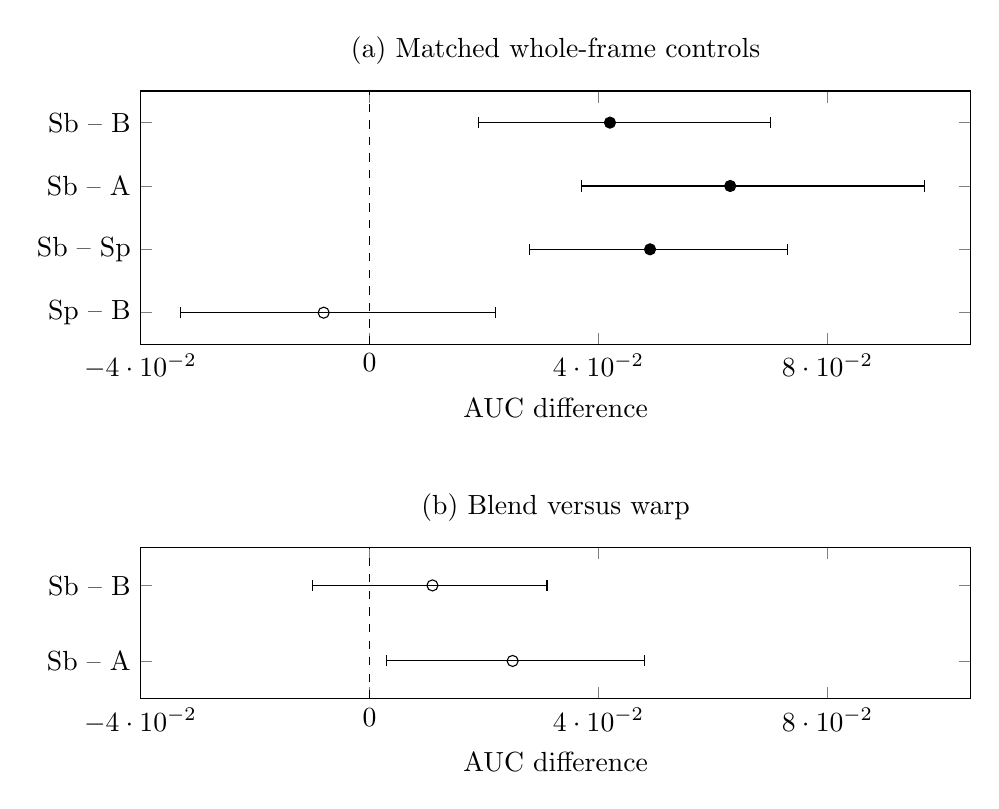
\begin{tikzpicture}
\begin{axis}[width=\linewidth,height=4.8cm,at={(0,0cm)},anchor=north west,scale only axis=false,title={(a) Matched whole-frame controls},xmin=-0.04,xmax=0.105,ymin=0.5,ymax=4.5,xtick={-0.04,0,0.04,0.08},xlabel={AUC difference},ytick={4,3,2,1},yticklabels={Sb -- B,Sb -- A,Sb -- Sp,Sp -- B}]
\addplot[dashed,mark=none] coordinates {(0,0.5) (0,4.5)};
\addplot[only marks,mark=*,error bars/.cd,x dir=both,x explicit] coordinates {(0.042,4) += (0.028000,0) -= (0.023000,0)};
\addplot[only marks,mark=*,error bars/.cd,x dir=both,x explicit] coordinates {(0.063,3) += (0.034000,0) -= (0.026000,0)};
\addplot[only marks,mark=*,error bars/.cd,x dir=both,x explicit] coordinates {(0.049,2) += (0.024000,0) -= (0.021000,0)};
\addplot[only marks,mark=o,error bars/.cd,x dir=both,x explicit] coordinates {(-0.008,1) += (0.030000,0) -= (0.025000,0)};
\end{axis}
\begin{axis}[width=\linewidth,height=3.5cm,at={(0,-5.8cm)},anchor=north west,scale only axis=false,title={(b) Blend versus warp},xmin=-0.04,xmax=0.105,ymin=0.5,ymax=2.5,xtick={-0.04,0,0.04,0.08},xlabel={AUC difference},ytick={2,1},yticklabels={Sb -- B,Sb -- A}]
\addplot[dashed,mark=none] coordinates {(0,0.5) (0,2.5)};
\addplot[only marks,mark=o,error bars/.cd,x dir=both,x explicit] coordinates {(0.011,2) += (0.020000,0) -= (0.021000,0)};
\addplot[only marks,mark=o,error bars/.cd,x dir=both,x explicit] coordinates {(0.025,1) += (0.023000,0) -= (0.022000,0)};
\end{axis}
\end{tikzpicture}

\fi
\caption{Development ranking gains. Top: two-person versus same-person whole-frame morphs, $D$-stratified, on development plus 80 person-overlap-screened hosts (seeds 408--412). Bottom: face-plus-halo blend-versus-warp diagnostic on FFHQ (seeds 403--407). Bars are 95\% component/block bootstrap intervals conditional on networks, not joint seed-and-host intervals. Filled/open points denote registered present/inconclusive verdicts. Panels use different data and resampling schemes.}
\label{fig:paired_evidence}
\end{figure}

\paragraph{Count-balanced follow-up.}
The post-freeze, development- and MAD22-informed follow-up reads all 30 networks (Sb, B, Sp, SpV, BN, BV; seeds 408--412), with no dropped seeds. Table~\ref{tab:count_balanced} reports its four registered outcomes. Primary OpenCV whole-frame ranking uses $D$-stratification on 100 development plus 80 screened test hosts; two-person whole-frame positives occur in training, but same-person whole-frame negatives do not. Secondary splice ranking uses the 80 screened hosts, unstratified as fixed before the read. Its 2,000 draws are all usable, unlike the stratified secondary diagnostic (37.7\% unreadable); primary stratification loses no draws. Both use paired host--partner component bootstraps (151/51 components), conditional on the five trained networks, without seed resampling.

\begin{table}[t]
\centering\small
\caption{Count-balanced development evidence: mean AUC differences and conditional 95\% component-bootstrap intervals. Positive-seed counts retain all five seeds.}
\label{tab:count_balanced}
\begin{tabular}{lccc}
\toprule
Pair & Gain & 95\% interval & Seeds $>0$ \\
\midrule
\multicolumn{4}{l}{Primary: whole-frame, $D$-stratified} \\
Sb $-$ SpV & +0.0481 & [0.0269, 0.0722] & 5/5 \\
BN $-$ BV & $-$0.0030 & [$-$0.0089, 0.0045] & 1/5 \\
\midrule
\multicolumn{4}{l}{Secondary: face splices, unstratified} \\
Sb $-$ SpV & +0.0818 & [0.0535, 0.1083] & 5/5 \\
BN $-$ BV & $-$0.0247 & [$-$0.0455, $-$0.0050] & 0/5 \\
\bottomrule
\end{tabular}
\end{table}

Sb--SpV supports replacing repeated native negatives with matched negatives plus 312 additional unique images in the full recipe. BN--BV lacks the registered $+0.03$ benefit on both outcomes; this is not equivalence to zero. Its adverse secondary effect contradicts the expected benefit: the 95\% interval is negative, but the 99.5\% sensitivity interval $[-0.0538,0.0031]$ crosses zero. Sb--SpV remains positive at 99.5\% on both outcomes; these sensitivities are not a familywise correction. Descriptive differences between pair effects are $+0.0511$ primary and $+0.1064$ secondary, with no interaction interval or significance test. Positive examples match only within pairs, so these differences do not isolate a universal requirement for splice positives. Independent numerical reconstruction exactly matched all 166 checks for the four outcomes; this verifies arithmetic, not external generalization.
% Sources: experiments/reviews/REVIEW_AB1_BATCHC_OPENCODE_20261114.md (full review);
% experiments/reviews/REVIEW_AB1_BATCHC_INDEPENDENT_REPRODUCTION_20261114.md (four-outcome reproduction).
% Reviewed output SHA256 9b73b148c57b9dbfbfdf60da2360aa9825ac7ddd8c42a94cd2fe137e21c802ea.
% Independent comparison SHA256 1b5a789ba01666c3c91e619c0049371ffcb85a1664536e23948461be8dc21bb7.
% Exact primary Sb-SpV +.048098592 [.026893408,.072238231]; BN-BV -.002992958 [-.008883478,.004497694].
% Exact secondary Sb-SpV +.081781250 [.053514957,.108347349]; BN-BV -.024656250 [-.045510204,-.005024836].

\paragraph{Storage sensitivity.}
Paired storage perturbations increase genuine false alarms by 26.5--38.5 percentage points for A at the trained small-image size, versus 0--4.5 points for Sb. At the untrained size, the corresponding ranges are 5.5--15.2 and 0--2.1 points. However, the registered test combines flag-rate and two-sided score-movement bounds. Sb passes five of five seeds at the trained size but only three at the untrained size: two failures arise from score movement toward genuine. The overall verdict is therefore inconclusive. We report attenuation of storage-induced false alarms, not removal of the shortcut.
% Source: AB1 result, registered R1 verdict and C2P per-seed rows.

\subsection{Development-exposed benchmark comparison}
\label{sec:mad22_results}
Table~\ref{tab:mad22_results} reports the frozen Sb networks on corrected MAD22~\cite{huber2022synmad}. No method met the registered freeze rule; the authors froze Sb by decision before these networks were benchmark-scored. The deciding endpoint was changed before that read from development-threshold errors to EER, because the training-source threshold flagged 96--98\% of unseen-source genuine photos. Its recipe was chosen after MAD22 results from earlier seeds were available; seeds 403--407 were new to benchmark evaluation. The genuine side comprises 204 FRLL photographs~\cite{debruine2017frll}. This is consequently a development-exposed benchmark evaluation, not an independent identity-level confirmation on FRLL. Released detectors are compared at their better raw-genuine or aligned-history form; SelfMAD's~\cite{ivanovska2025selfmad} raw form has the lowest four-family point mean among MADation B/16, MADation L/14, MixFaceNet-MAD and SelfMAD, each in raw-genuine and history-matched forms. This comparator is held fixed in bootstrap draws; it is not selected separately for each table row.
% Sources: experiments/FINAL_sealed-benchmark-read/result.md, labels and primary endpoint; prereg.md C1--C3 (freeze and endpoint amendments).

\begin{table}[t]
\centering\small
\caption{Corrected MAD22 EER (\%), lower is better. Sb uses the registered history-matched form and is averaged over five seeds. SelfMAD uses raw genuine photographs. MAD22 influenced recipe development.}
\label{tab:mad22_results}
\begin{tabular}{lrr}
\toprule
Family ($n$ morphs) & Sb & SelfMAD \\
\midrule
OpenCV (984) & 2.26 & 1.02 \\
Webmorph (500) & 10.39 & 13.73 \\
MIPGAN-I (1,000) & 0.57 & 2.45 \\
MIPGAN-II (999) & 0.28 & 1.70 \\
\midrule
Four-family mean & 3.37 & 4.72 \\
Landmark-only mean & 6.32 & 7.37 \\
\bottomrule
\end{tabular}
\end{table}

The four-family difference is $-1.4$ percentage points, with a two-level 95\% interval of $[-3.51,0.98]$. Each of 2,000 paired bootstrap draws resamples the 102 contributor persons and five seed indices. A genuine photo receives its person's multinomial count; a morph receives the product of both contributors' counts. Common draws serve all detectors and families. The registered one-point non-inferiority criterion narrowly passes: its bootstrap tail probability is 0.02499 against 0.025; one additional exceedance among 2,000 replicates changes the verdict. Superiority is not established. The landmark-only difference is $-1.0$ points $[-4.7,3.0]$ and is not separated. Half of the primary average comprises GAN families whose identity specificity remains unresolved by our rendering controls. FaceMorpher was excluded from this endpoint because morph-free networks achieve zero EER on that cell. Finally, EER is not the fixed-threshold error: Webmorph attack misses at the own rule range from 24--58\%, while genuine false alarms range from 0--2.5\%. These results support competitive discrimination alongside, rather than proof against, remaining shortcuts.
